%!TEX root = ../var.tex
\begin{zam}
\label{zam:16.1}
Пусть $\xi_1 , \xi_2$ -- случайные величины с совместной плотностью вероятности $f_{\xi_1 ,\xi_2} (x_1 , x_2 )$. Построим с помощью функции $g : \mathbb{R}^2 \to \mathbb{R}$ случайную величину $\eta = g(\xi_1 , \xi_2 )$. Требуется найти функцию распределения $F_\eta (y)$ и плотность вероятности $f_\eta (y)$ случайной величины $\eta$.
\end{zam}

\begin{lemma}
\label{lemma:16.2}

Пусть $y \in \mathbb{R}$, и область $D_y \subseteq \mathbb{R}^2$ состоит из точек $(x_1 , x_2 )$, удовлетворяющих неравенству $g(x_1 , x_2 ) \leq y$, т.е. $$D_y = \{(x_1 , x_2 ) \in \mathbb{R}^2 | g(x_1 , x_2 ) \leq y\}$$. Тогда случайная величина $\eta = g(\xi_1 , \xi_2 )$ имеет функцию распределения
\begin{gather*}
	F_\eta (y) = \iint\limits_{D_y}f_{\xi_1,\xi_2} (x_1 , x_2 ) dx_1 dx_2
\end{gather*}
\end{lemma}

\begin{proof}
\begin{gather*}
	F_\eta (y) = \P ( g(x_1 , x_2 ) \leq y ) = \P( (x_1 , x_2 ) \in Dy )= \iint\limits_{D_y}f_{\xi_1 ,\xi_2} (x_1 , x_2 ) dx_1 dx_2
\end{gather*}

где последнее равенство следует их того, что вероятность попадания случайного вектора $(x_1 , x_2 )$ в область $D_y$ равна объёму цилиндра, ограниченного сверху графиком плотности вероятности, а снизу -- областью $D_y$.
\end{proof}

\begin{figure}[H]
	\centering
	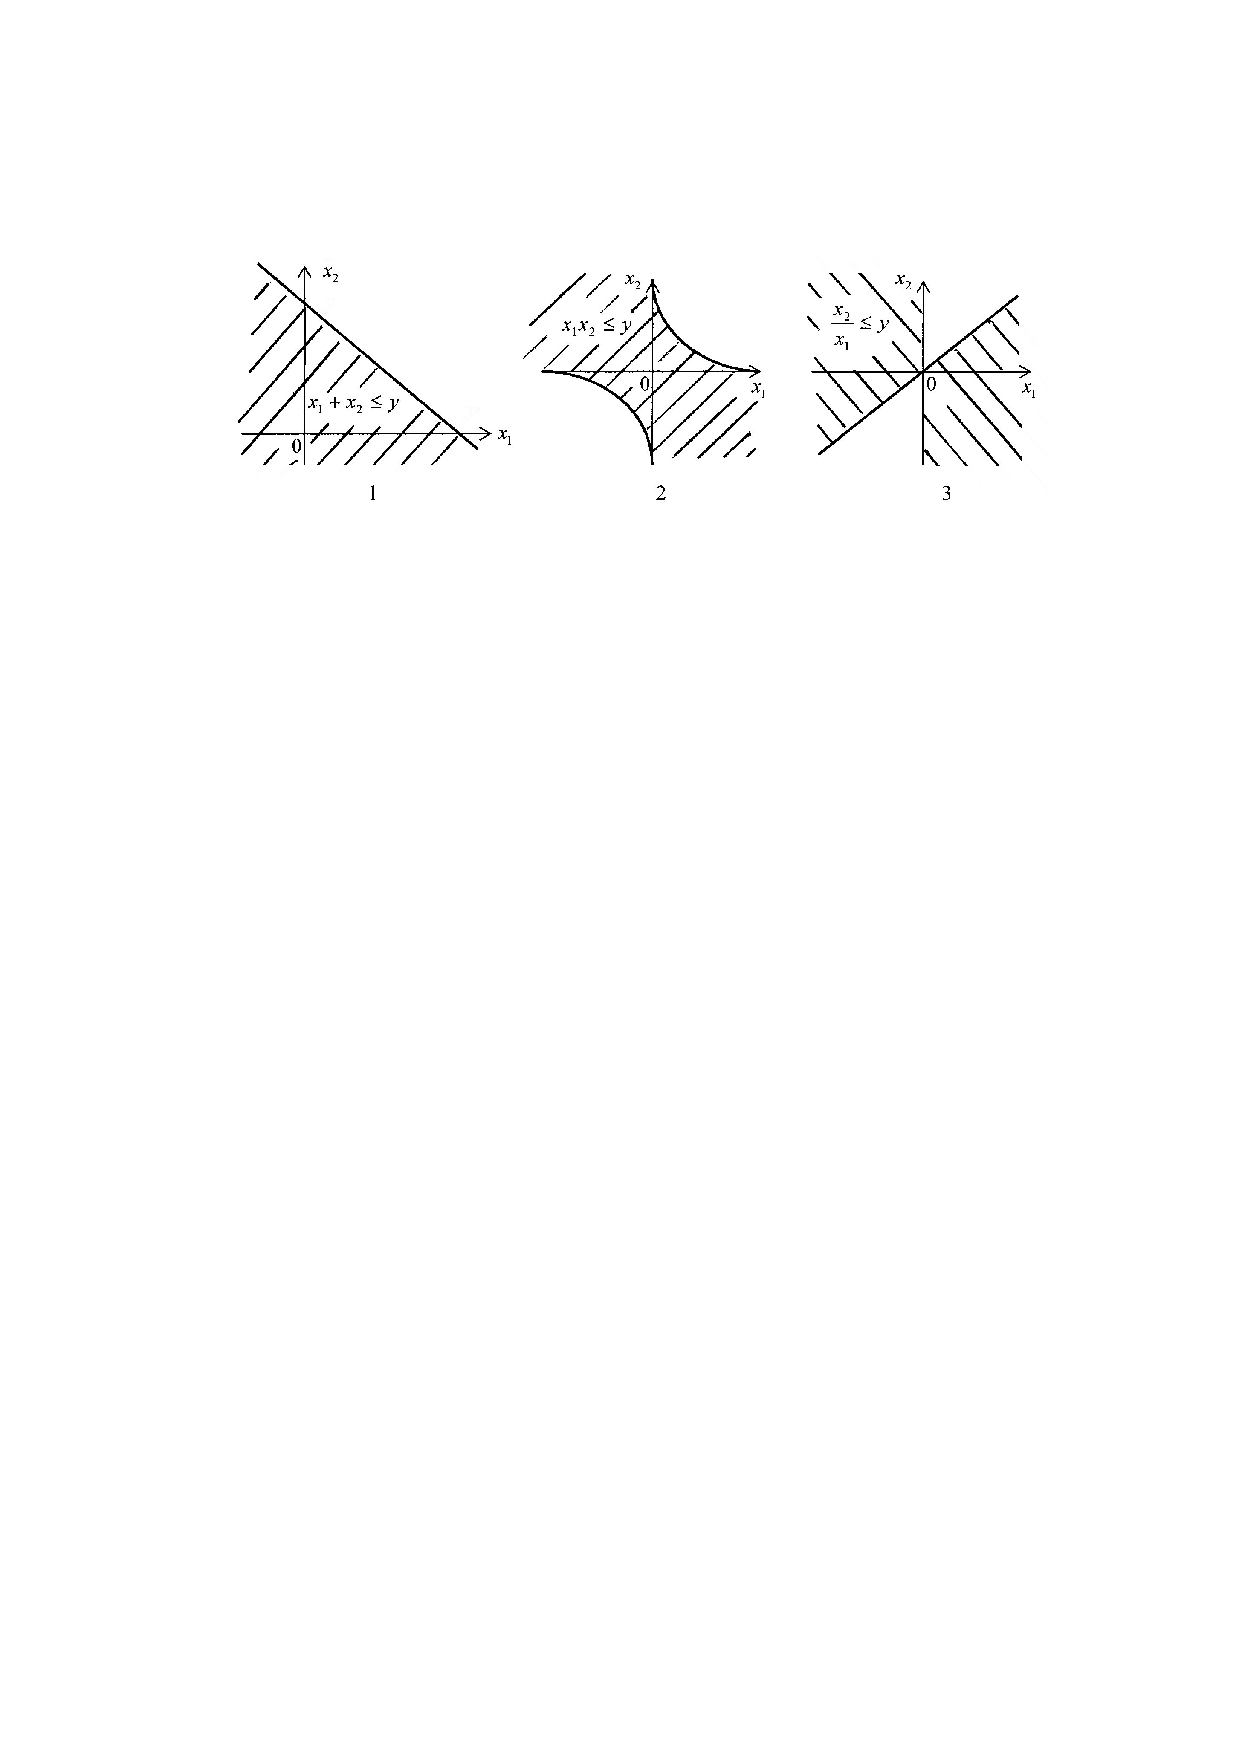
\includegraphics[]{pic/pic22}
	\caption{Случайные функции суммы, произведения и частного}
	\label{fig22}
\end{figure}

\begin{lemma}[Распределение суммы]
\label{lemma:16.3}
Пусть $\eta = \xi_1 + \xi_2$, тогда

\begin{gather*}
	F_\eta (y) = \P ( \eta \leq y ) = \P(x_1+x_2 \leq y )=
	\int\limits_{-\infty}^{\infty}\left(
		\int\limits_{-\infty}^{y-x_1 } f_{\xi_1,\xi_2} (x_1 , x_2 ) dx_2
	\right)dx_1
\end{gather*}
\end{lemma}
\begin{proof}
Воспользуемся леммой \ref{lemma:16.2} для функции $g(x_1 , x_2 )=x_1 + x_2$. 

Заменим двойной интеграл по области $D_y = \{(x_1 , x_2 ) \in \mathbb{R}^2 | x_1 +
x_2 \leq y\}$ (см. рис. \ref{fig22}.1) на повторный, получим требуемый результат.	
\end{proof}

\begin{lemma}[Распределение произведения]
\label{lemma:16.4}
Пусть $\eta = \xi_1 \xi_2$ , тогда

\begin{gather*}
	F_\eta (y) = \P ( x_1x_2 \leq y ) =
	\int\limits_{-\infty}^{0}\left(
		\,\,\int\limits_{y/x_1}^{\infty} f_{\xi_1,\xi_2} (x_1, x_2 ) dx_2
	\right)dx_1+\\+
	\int\limits_{0}^{\infty}\left(
		\,\,\int\limits^{y/x_1}_{-\infty} f_{\xi_1,\xi_2} (x_1, x_2 ) dx_2
	\right)dx_1
\end{gather*}
\end{lemma}

\begin{proof}
	Воспользуемся леммой \ref{lemma:16.2} для функции $g(x_1 , x_2 ) = x_1 x_2$.

Область $D_y = \{(x_1 , x_2 ) \in \mathbb{R}| x_1 x_2 \leq y\}$ показана на рис. \ref{fig22}.2. Переходя от двойного интеграла к повторному, получим требуемый результат.
\end{proof}

\begin{lemma}[Распределение частного]
\label{lemma:16.5}
Пусть $\eta = \frac{\xi_2}{\xi_1}$, тогда
\begin{gather*}
	F_\eta (y) = \P ( \frac{x_2}{x_1} \leq y ) =
	\int\limits_{-\infty}^{0}\left(
		\,\,\int\limits_{yx_1}^{\infty} f_{\xi_1,\xi_2} (x_1, x_2 ) dx_2
	\right)dx_1+\\+
	\int\limits_{0}^{\infty}\left(
		\,\,\int\limits^{yx_1}_{-\infty} f_{\xi_1,\xi_2} (x_1, x_2 ) dx_2
	\right)dx_1
\end{gather*}
\end{lemma}
\begin{proof}
Доказательство. Воспользуемся леммой \ref{lemma:16.2} для функции $g(x_1 , x_2 ) = \frac{x_2}{x_1}$.

Область $D_y = \{(x_1 , x_2 ) \in \mathbb{R}^2  \frac{x_2}{x_1} \leq y\}$ показана на рис. \ref{fig22}.3. Переходя от двойного интеграла к повторному, получим требуемый результат.
\end{proof}

\begin{lemma}[О свёртке]
\label{lemma:16.6}
	Если случайные величины $\xi_1$ и $\xi_2$ независимы
и имеют плотности вероятности соответственно $f_{\xi_1} (x_1 )$ и $f_{\xi_2} (x_2 )$, то плотность вероятности суммы $\eta = \xi_1 + \xi_2$ равна свёртке плотностей $f_{\xi_1}$ и $f_{\xi_2}$:
\begin{gather*}
	f_\eta (t)=f_{\xi_1+\xi_2}(t)=\int\limits_{-\infty}^{\infty} f_{\xi_1} (u)f_{\xi_2} (t - u) du=
	\int\limits_{-\infty}^{\infty} f_{\xi_2}(u)f_{\xi_1} (t - u) du
\end{gather*}
\end{lemma}

\begin{proof}
Воспользуемся леммой \ref{lemma:16.3}
\begin{gather*}
	F_\eta (y) =
	\int\limits_{-\infty}^{\infty}\left(
		\int\limits_{-\infty}^{x-x_1 } f_{\xi_1,\xi_2} (x_1 , x_2 ) dx_2
	\right)dx_1=
	\int\limits_{-\infty}^{\infty}\left(
		\int\limits_{-\infty}^{x-x_1 } f_{\xi_1}(x_1)f_{\xi_2}(x_2) dx_2
	\right)dx_1
\end{gather*}

Сделаем в последнем интеграле замену переменной: $x_2 = t - x_1$ , $dx_2 = dt$.
При этом $x_2 \in (-\infty, x - x_1 )$ перейдёт в $t \in (-\infty, x)$. В последнем интеграле меняем порядок интегрирования и получаем:
\begin{gather*}
	\int\limits_{-\infty}^{\infty}\left(
		\int\limits_{-\infty}^{x} f_{\xi_1}(x_1)f_{\xi_2}(t-x_1) dt
	\right)dx_1=
	\int\limits_{-\infty}^{x}\overbrace{\left(
		\int\limits_{-\infty}^{\infty} f_{\xi_1}(x_1)f_{\xi_2}(t-x_1) dx_1
	\right)}^{f_{\xi_1+\xi_2}(t)}dt=
\end{gather*}

Итак, мы представили функцию распределения $F_\eta (x) = F_{\xi_1 +\xi_2} (x)$ в виде $\int\limits_{-\infty}^{x} f_{\xi_1 +\xi_2} (t) dt$, где

\begin{gather*}
	f_{\xi_1 +\xi_2} (t)=\int\limits_{-\infty}^{\infty} f_{\xi_1}(x_1)f_{\xi_2}(t-x_1) dx_1=\int\limits_{-\infty}^{\infty} f_{\xi_1}(u)f_{\xi_2}(t-u) du
\end{gather*}

Второе равенство теоремы получается из первого, если всюду в доказательстве поменять местами индексы 1 и 2.
\end{proof}

\begin{definition}
\label{def:16.7}
Если две независимые случайные величины имеют одно и то же распределение (возможно, с разными параметрами), и их сумма имеет то же самое распределение, то распределение называется устойчивым относительно суммирования.
\end{definition}

\begin{zam}
\label{zam:16.8}
Следующие леммы могут быть доказаны непосредственно с помощью формулы свёртки, однако более короткие доказательства будут приведены в параграфе \ref{par:25}, используя характеристические функции.
\end{zam}

\begin{lemma}
\label{lemma:16.9}
	Пусть независимые случайные величины $\xi_n$ и $\xi_m$ имеют
биномиальное распределение (см. определение \ref{def:12.8}), с параметрами $n$ и $m$ и вероятностью <<успеха>>  p, тогда случайная величина $\xi_n + \xi_m$ имеет биномиальное распределение $\xi_{n+m}$ . Другими словами, биномиальное распределение является устойчивым относительно суммирования.
\end{lemma}

\begin{lemma}
\label{lemma:16.10}
Пусть независимые случайные величины $\xi$ и $\eta$ имеют
нормальное распределение (см. определение \ref{def:12.8}), и имеют соответственно математические ожидания $a_1$ и $a_2$ и дисперсии $\sigma_1^2$ и $\sigma_2^2$, тогда случайная величина $\xi + \eta$ имеет нормальное распределение с математическим ожиданием $a_1 + a_2$ и дисперсией $\sigma_1^2+\sigma_2^2$. Другими словами, нормальное распределение является устойчивым относительно суммирования.	
\end{lemma}

\textbf{Пример}. Товарняк состоит из 100 вагонов. Масса (измеряемая в тоннах т) произвольного вагона -- случайная величина, распределенная по нормальному закону с средним значением 65 тонн и среднеквадратичным отклонением 9 тонн. Локомотив может везти состав массой не более 6600 тонн, в противном случае необходимо прицеплять второй локомотив. Найти вероятность того, что второй локомотив не потребуется.

\textit{Решение}. По лемме \ref{lemma:16.10} имеем $a = a_1 + \ldots + a_{100} = 65 \ldots 100 = 6500$, $\sigma = \sigma_1^2 +\ldots+\sigma_{100}^2=81\cdot100 = 8100$.

Вероятность того, что второй локомотив не потребуется, составляет $\P(\xi \leq 6600) = F_\xi (6600)=\frac{1}{2}+\Phi(\frac{x-a}{\sigma})=\frac{1}{2}+\Phi(\frac{6600-6500}{90})=\frac{1}{2}+\Phi(\frac{10}{9})\approx\frac{1}{2}+\Phi(1.11)\approx0.87$, где $\Phi(z) = \frac{1}{\sqrt{2\pi}}\int\limits_0^z e^{-t^2/2}dt$ -- табличный интеграл вероятности нормального распределения. 